\section{Test Driven Development}

\begin{frame}{(Test Driven Development)} 
    \framesubtitle{Program CSE tests first}
        \vfill

        TDD\footnote{Freeman, Steve, and Nat Pryce. Growing object-oriented software, guided by tests. Pearson Education, 2009.} for CSE
        \begin{itemize}
            \item Define verification and validation tests at the start.
            \item Focus placed the final result: interpolation, integration, discretization, PDE solution, physics. 
            \item Top-down, instead of bottom-up test coverage.
            \item Don't go overboard with unit-tests \faGraduationCap: extend unit-tests when debugging a failing CSE test.  
            \item Focus kept on tests with real-world (publication) input. 
        \end{itemize}

\end{frame}

\begin{frame}{(Test Driven Development)} 
    \framesubtitle{Verification and validation tests define the Application Programming Interface}
        \vfill

    \begin{itemize}
        \item \textbf{New code}: it is easier to program the API you wish for, if you are its first user. 
            \begin{itemize}
                \item Make the class interface easy to use correctly and difficult to use incorrectly\footnote{Scott Meyers. 2014. Effective Modern C++: 42 Specific Ways to Improve Your Use of C++11 and C++14 (1st. ed.). O'Reilly Media, Inc.}.
                \item Reduce number of function arguments, single responsibility, clear naming, ... 
            \end{itemize}
        \item \textbf{Legacy code}: extend existing API without modification. 
            \begin{itemize}
                \item OpenFOAM: understanding class hierarchies, \textit{finding a base class with Runtime Type Selection and a virtual function to overload.}
            \end{itemize}
        \item \textbf{The test application is the solver application with a different input.}
            \begin{itemize}
                \item If possible, testing and solution is done by the same code.  
                \item This prevents code duplication. 
                \item Data output and additional checks can be disabled by (compile-time) options.
            \end{itemize}
    \end{itemize}

\end{frame}


\begin{frame}{Test Driven Development} 
    \framesubtitle{Jupyter notebooks}

    \vfill
    Jupyter notebooks\footnote{\href{https://jupyter.org/}{https://jupyter.org/}}
    \begin{itemize}
        \item \textbf{Documentation}: geometry, initial and boundary conditions, error norms, comparison data.
        \item \textbf{Processing}: verification errors (conservation, convergence, stability), validation errors. 
        \item \textbf{Result analysis}: very straightforward, interactive, remote.
    \end{itemize}
\end{frame}

\begin{frame}{Test Driven Development} 
    \framesubtitle{(Parameter tests)}
    
    \vfill
    \begin{center}
            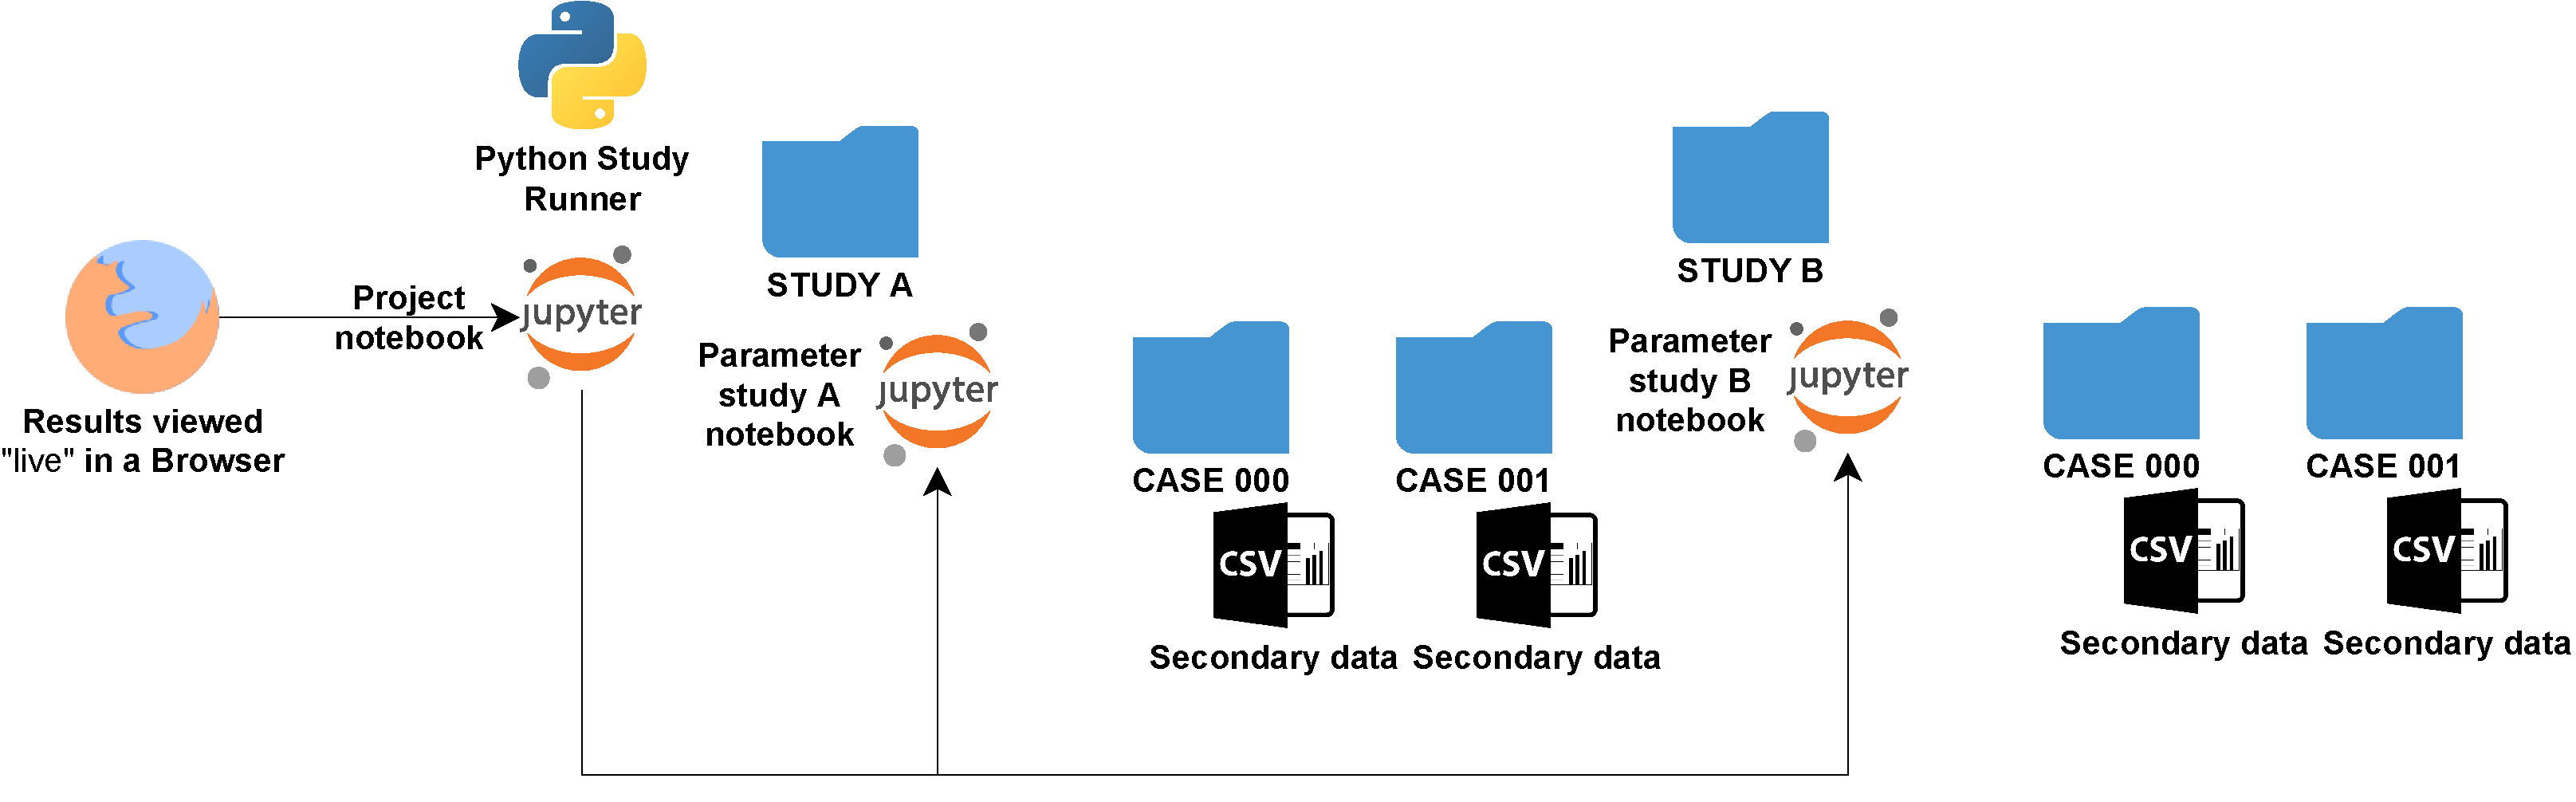
\includegraphics[width=0.9\textwidth]{figures/Cluster-Parameter-Study-Organization.pdf}
    \end{center}
\end{frame}

\begin{frame}{Test Driven Development} 
    \framesubtitle{Parameter tests: primary data (simulation results) organization}

    \begin{itemize}
        \item The quality of CSE software is measured using verification and validation data. 
        \item Effective comparison with others (previous versions) hinges on data organization.
    \end{itemize}
    
    \vfill
    \begin{itemize}
        \item \textbf{Legacy code}: 
            \begin{itemize}
                \item use the existing folder structure and parameterization tools \faGraduationCap,
                \item The mapping (case000) $\to$ (parameter vector) must be stored (YAML, ...)
            \end{itemize}
        \item \textbf{New code}: 
            \begin{enumerate}
                \item Simple folder and file structure \faGraduationCap
                \item HDF5\footnote{\url{https://www.hdfgroup.org/solutions/hdf5}} or other open data format.
                \item Alternative to HDF5: \textbf{ExDir}\footnote{Dragly, Svenn-Arne, et al. "Experimental Directory Structure (Exdir): An alternative to HDF5 without introducing a new file format." Frontiers in neuroinformatics 12 (2018): 16.} 
            \end{enumerate}
    \end{itemize}

\end{frame}


\begin{frame}{Test Driven Development} 
    \framesubtitle{Parameter tests: secondary data (tables and diagrams) organization}

    \href{https://pandas.pydata.org/}{pandas.MultiIndex} CSV with metadata for secondary data
    \begin{itemize}
        \item \texttt{pandas.MultiIndex} saved in "metadata columns". 
        \item \textcolor{red}{\textbf{Metadata is repeated}}: not an issue for the small secondary data! 
        \item Metadata in columns $\to$ \texttt{pandas.MultiIndex} $\to$ strongly simplified data analysis. 
        \item \textbf{Direct readable export of tables to LaTex!}
    \end{itemize}

    \footnotesize

    \begin{tabular}{llllll}
        \toprule
        {} &         H &     L\_INF &  O(L\_INF) &  EPSILON\_R\_EXACT\_MAX &  O(EPSILON\_R\_EXACT\_MAX)  \\ 
        VELOCITY\_MODEL &           &           &           &                      &                        \\ 
        \midrule
        \textcolor{red}{\textbf{SHEAR\_2D}}       &  0.125000 &  0.032961 &  1.833407 &             0.032961 &                1.833407 \\ 
        \textcolor{red}{\textbf{SHEAR\_2D}}       &  0.062500 &  0.009249 &  1.955529 &             0.009249 &                1.955529 \\ 
        \textcolor{red}{\textbf{SHEAR\_2D}}       &  0.031250 &  0.002385 &  1.988745 &             0.002385 &                1.988745 \\ 
        \textcolor{red}{\textbf{SHEAR\_2D}}       &  0.015625 &  0.000601 &  1.997178 &             0.000601 &                1.997178 \\ 
        \textcolor{red}{\textbf{SHEAR\_2D}}       &  0.007813 &  0.000150 &  1.999294 &             0.000150 &                1.999294 \\ 
        \textcolor{red}{\textbf{SHEAR\_2D}}       &  0.003906 &  0.000038 &  1.999294 &             0.000038 &                1.999294 \\ 
        \bottomrule
    \end{tabular}

\end{frame}
